For å vurdere lønnsomheten til prosjektet har vi utarbeidet kontantstrømmer prosjektet vil generere og kontantstrømmer basert på å fortsette med nåværende teknologi. Deretter har vi beregnet differansekontantstrømmer ved å sammenligne inntekter og kostnader de to alternativene medfører. Netto nåverdi-analysen baseres på sistnevnte beregning. Figuren nedenfor viser et utdrag fra differansekontantstrømmen i årene før el-ovnen er klar til produksjon, de første tre årene med produksjon og de to siste. Fullstendig kontanstrømmer finnes i vedlegg \ref{fig:nnvelovn}, \ref{fig:nnvnow}, \ref{fig:nnvdiff}.

\begin{table}[H]
  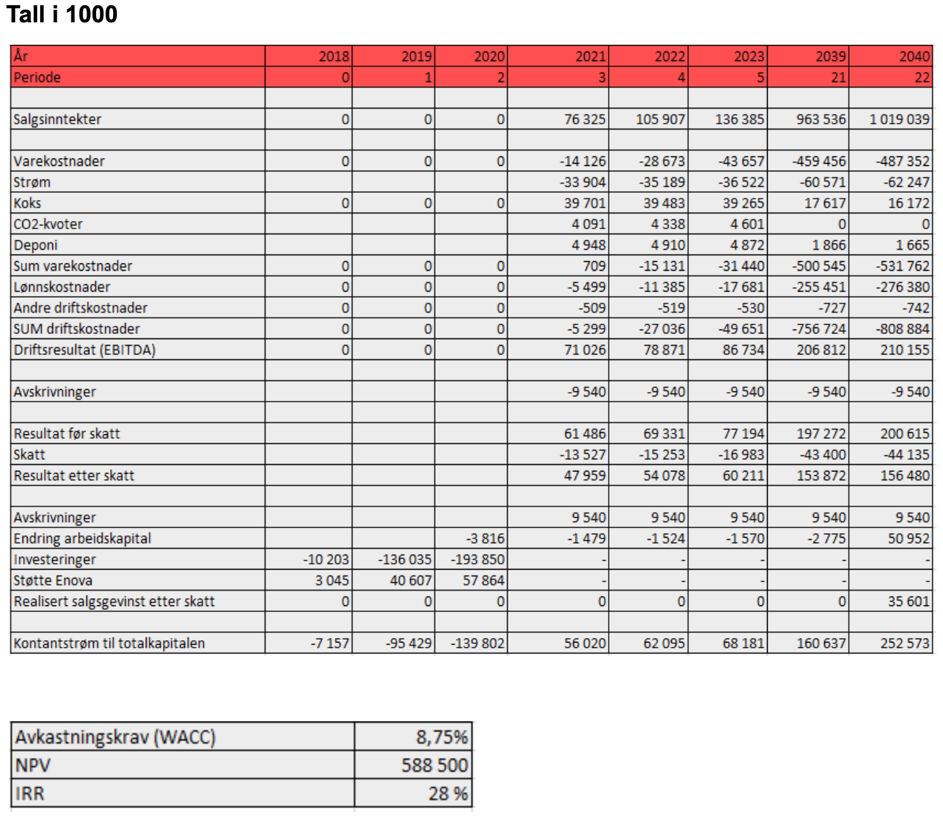
\includegraphics[width=\linewidth]{tabeller/lonnsomhet.png}
  \caption{Rockwool kontantstrømmer}
  \label{tbl:lonnsomhet}
\end{table}

Analysen viser til en positiv netto nåverdi på 588.500.000 kroner ved et totalkapitalkrav på 8,75\%. Den totale avkastningen på prosjektet er 28,32\% og vises gjennom internrenten. Dette gir en ekstraordinær avkastning på 19,57\% utover totalkapitalkravet.